\documentclass[tikz]{standalone} 
\usetikzlibrary{arrows, decorations.markings}
\usetikzlibrary{arrows.meta, positioning, tikzmark}
\begin{document}

   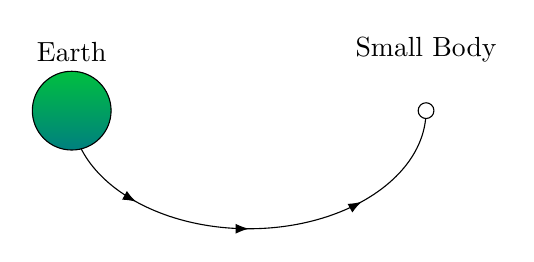
\begin{tikzpicture}[>=Latex,
                       mydeco/.style = {decoration = {markings, 
                                                       mark = at position #1 with {\arrow{>}}}
                                       }
                      ]

    \coordinate (ast) at (1.5, 0);
    \coordinate (earth) at (-3, 0);
    \node[above, yshift=0.5cm] at (earth) {Earth};
    \node[above, yshift=0.5cm] at (ast) {Small Body};
    % \draw[postaction = {mydeco=0.0416 ,decorate}, 
    % postaction = {mydeco=0.58333 ,decorate}] (0,0) circle (3cm);

    % \draw[postaction = {mydeco=0.375 ,decorate}, 
    % postaction = {mydeco=0.875 ,decorate}] (0,0) circle (1.5cm);


    \draw[postaction = {mydeco=0.25 ,decorate}, 
    postaction = {mydeco=0.5 ,decorate},
    postaction = {mydeco=0.75, decorate}] (earth) arc (180:360:2.25cm and 1.5cm)
    node[midway, above] {};

    \draw[fill = white] (ast) circle (0.1cm);

    \filldraw[top color = green!75!blue, bottom color = blue!50!green] (earth) circle (0.5cm);

   \end{tikzpicture}

\end{document}
